\subsection*{6. Final Form of the Wavefunction}

The complete fermionic wavefunction for the considered state is therefore:


\begin{equation}
	\Psi_F(x_1, x_2, t) = \frac{1}{\sqrt{2}}
	\left[
		\sin\left(\frac{n\pi x_1}{L}\right)\sin\left(\frac{\kappa\pi x_2}{L}\right)
		- \sin\left(\frac{\kappa\pi x_1}{L}\right)\sin\left(\frac{n\pi x_2}{L}\right)
	\right]
	e^{-iEt/\hbar},
\end{equation}
with $E$ given above.

\begin{figure}[h!]
	\centering
	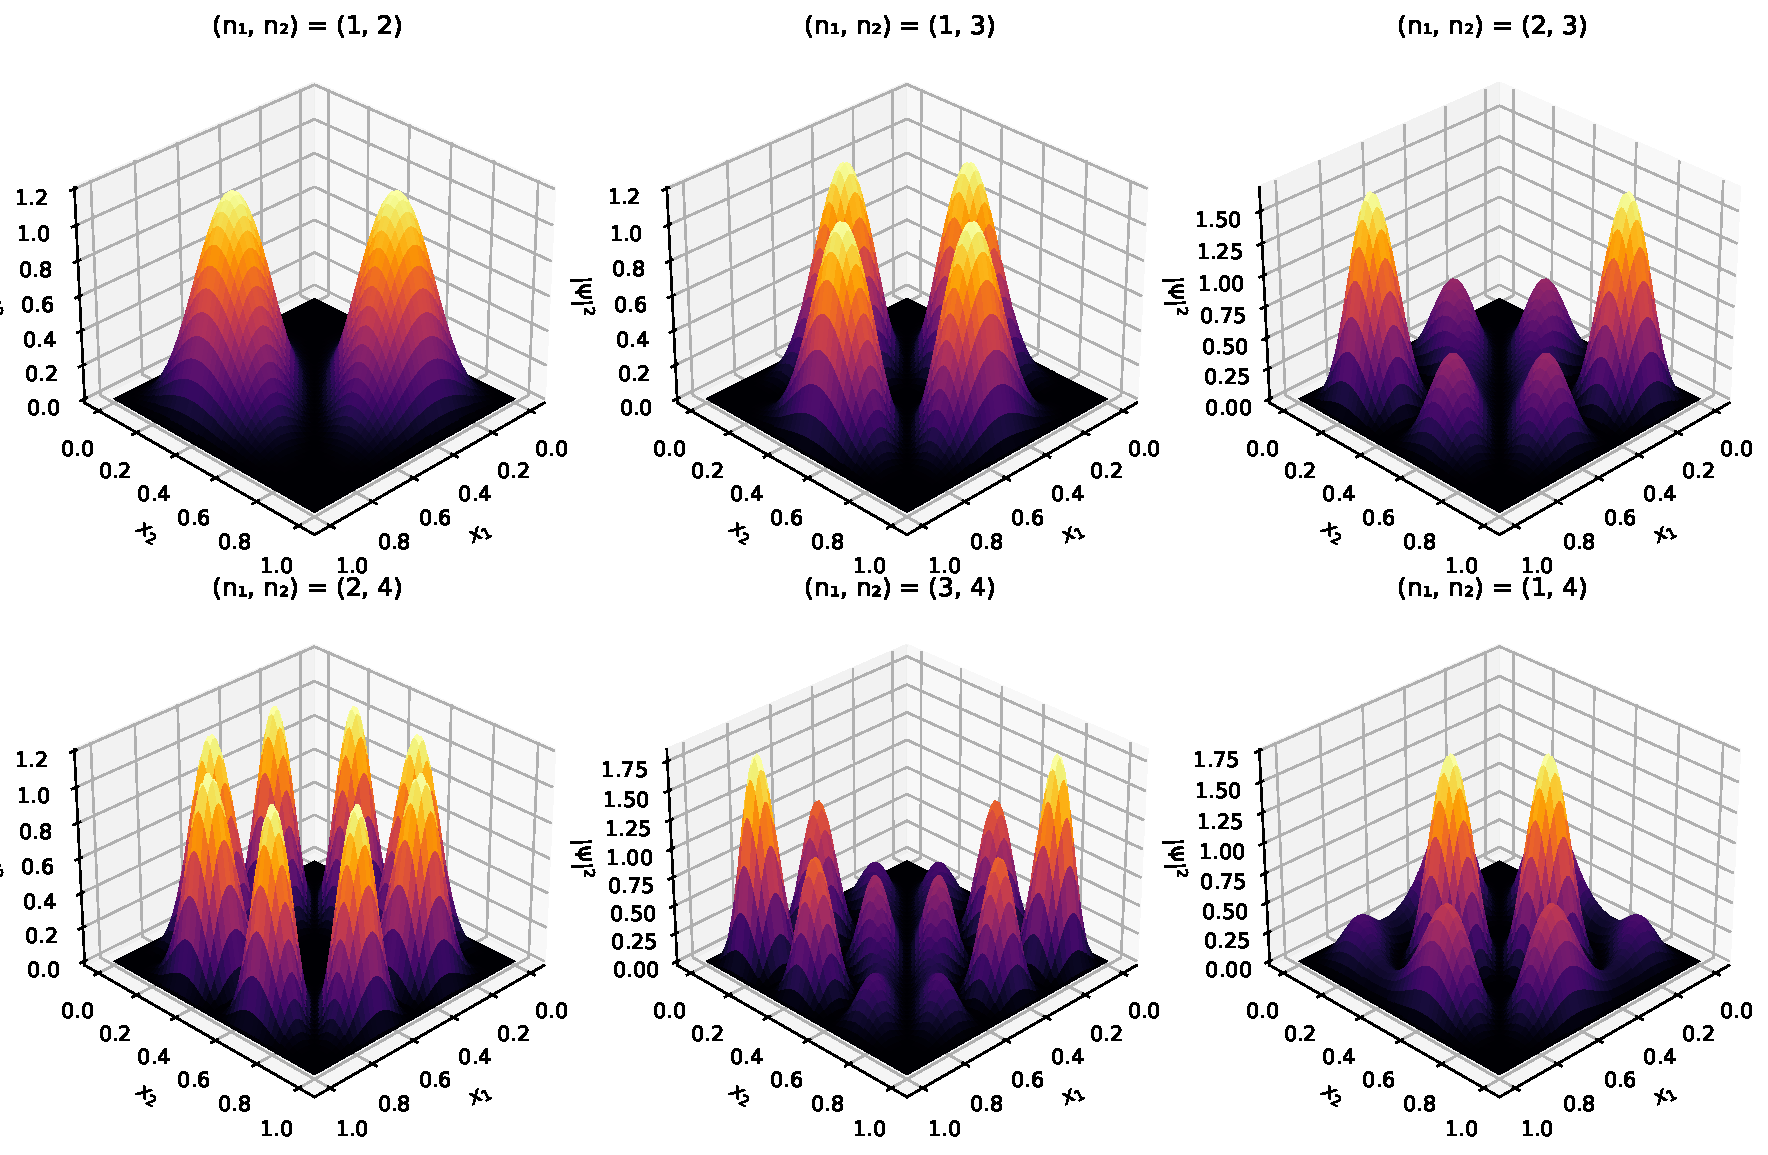
\includegraphics[width=0.9\textwidth]{ figures/fermions_3D_collage-1.pdf}
	\caption{Probability density $|\Psi_F(x_1, x_2)|^2$ for six antisymmetric two-fermion configurations
		$(n,\kappa) = (1,2), (1,3), (2,3), (2,4), (3,4), (1,4)$.
	The antisymmetric nature of the wavefunction enforces $\Psi_F(x_1 = x_2) = 0$, reflecting the Pauli exclusion principle.}
	\label{fig:fermion_3D_collage}
\end{figure}


\section{Remarks and Validity}

The derivation above is valid for the antisymmetric spatial sector (fermions) and for the idealized contact interaction represented by the delta potential. For bosonic states, the delta interaction generally yields nontrivial corrections to energy eigenvalues and must be treated using either regularization methods or matching conditions across the line $x_1=x_2$. The present fermionic ansatz trivially nullifies the delta contribution because of the vanishing of the wavefunction at coincidence points.
